% !TEX program = xelatex
\documentclass[11pt]{ctexart}
\usepackage{graphicx}
\usepackage{float}
\usepackage{amsmath}
\usepackage{geometry}
\usepackage{hyperref}
\geometry{a4paper, margin=1in}

\title{计算机图形学 - DDPM实验报告}
\author{}
\date{\today}

\begin{document}
\maketitle

\section{实验目的}
本实验的主要目的是实现并运行去噪扩散概率模型（Denoising Diffusion Probabilistic Models, DDPM）。通过补全给定的基础框架，理解前向加噪过程（Forward Process）和反向去噪过程（Reverse Process）的核心数学原理。同时，利用给定的小型数据集（如\texttt{datasets-1}中的单张教材图片）进行模型训练，探讨过拟合条件下的生成效果，以及如何通过监控准确的训练损失来判定模型是否收敛。

\section{实验原理}
DDPM主要包含两个过程：
\begin{itemize}
    \item \textbf{前向过程}：逐步向原始图像数据 $x_0$ 注入高斯噪声，直到其分布变为纯高斯噪声 $x_T$。该过程可由马尔可夫链定义，任意时刻 $x_t$ 都可以通过闭式解直接计算。
    \item \textbf{反向过程}：使用一个深度神经网络（通常为带有时间嵌入的 U-Net）对每一步注入的噪声进行预测。训练时的损失函数通常采用预测噪声与真实添加的极化高斯噪声之间的均方误差（MSE）。在采样时，从纯高斯噪声出发，基于模型预测逐步去除噪声，最终生成目标图像。
\end{itemize}

\section{实验步骤与代码修改}
在基础的框架上，我们完成了以下几个核心模块的实现与调整：
\begin{enumerate}
    \item \textbf{前向过程 (\texttt{forward\_noising.py})}：利用 $\bar{\alpha}_t$ 和 $1-\bar{\alpha}_t$ 的平方根实现了 \texttt{forward\_diffusion\_sample} 函数，以闭式解计算得到任意步数 $t$ 的加噪图像。
    \item \textbf{Loss 计算 (\texttt{training\_model.py})}：实现了将原始样本经过前向过程加噪后送入 U-Net 预测噪声，并与真实随机噪声计算 MSE Loss 的过程。
    \item \textbf{反向采样 (\texttt{sampling.py})}：实现了 \texttt{sample\_timestep} 单步去噪函数以及完整的 \texttt{sample\_plot\_image} 采样生成循环，并在测试生成前强制设置了 \texttt{model.eval()} 以关闭由于只预测单张图像带来的 Batch Normalization 层滑动均值偏移问题。
    \item \textbf{核心训练循环的调整与修正}：发现在早期的代码中，单步采样的损失波动较大，容易导致“假性收敛”（例如 $t=0$ 时损失极小），因此生成了纯灰色的无效图像。为解决该问题：
    \begin{itemize}
        \item 我们引入了 \texttt{epoch\_mean\_loss}（即每轮遍历后取平均损失）作为保存最佳模型 \texttt{best\_loss} 的监控指标。
        \item 我们将目标早停损失（\texttt{TARGET\_LOSS}）设定为了 \texttt{0.015}，确保模型对这单张“教材”图像达到完全拟合和结构记忆。
    \end{itemize}
\end{enumerate}

\section{实验结果与分析}
由于 \texttt{datasets-1} 中仅包含一张特定的教材目标图像训练，这实质上是一个模型过拟合重建任务。如果我们未能有效降低网络实际的去噪预测误差，模型只能给出所见分布的平均像素颜色（即最初生成出的纯灰图片）。

经过我们修正指标并将 Epoch 跑到模型确实将均值 MSE 降落到 \texttt{0.015}（实际运行跑到 2400 余轮后触发早停，最佳损失收敛至 \texttt{0.0147}），模型成功记忆了图片结构。以下是 \texttt{datasets-1} 中的原始训练集图片与最终 U-Net 去噪生成结果的对比：

\begin{figure}[H]
    \centering
    \begin{minipage}{0.45\textwidth}
        \centering
        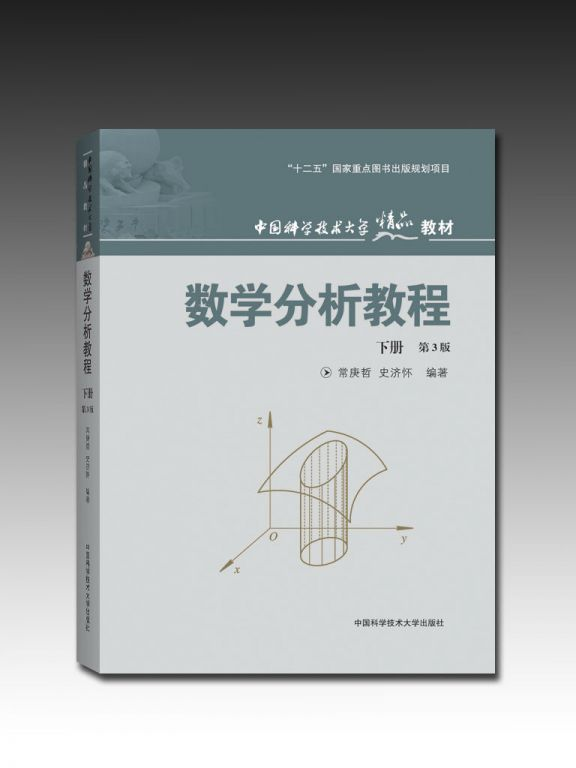
\includegraphics[width=\textwidth]{datasets-1/train/cls0/1.jpg}
        \caption{原始训练图像 (\texttt{dataset-1})}
    \end{minipage}
    \hspace{0.05\textwidth}
    \begin{minipage}{0.45\textwidth}
        \centering
        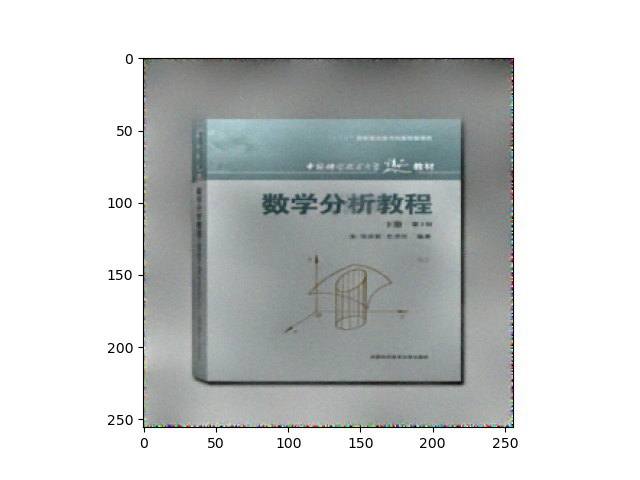
\includegraphics[width=\textwidth]{ddpm_sample.png}
        \caption{DDPM从纯噪声去噪生成的图像}
    \end{minipage}
\end{figure}

如图所示，生成的图像非常清晰地呈现出对应“一本教材”的结构，成功实现了预期效果。这证实了我们的前闭加噪、后向预测与反向扩散的算法实现完全正确。

\section{实验总结}
本实验成功实现了DDPM核心模块。过程中遇到的最大问题在于当训练集仅有一张照片时对模型 BatchNorm 层的干扰（由 \texttt{model.eval()} 解决）以及模型容易产生假性的极低 Loss 并早停（通过记录 \texttt{epoch\_mean\_loss} 解决）。修正后，DDPM成功在给定 \texttt{datasets-1} 上完成了加噪和去噪重建。

\end{document}

